\section{Brick Manufacturing Process}
% Information about the manufacturing process of bricks.

\subsection{Block Diagram}
% Description of the block diagram of the brick manufacturing process.
\begin{figure}[h]
  \centering
  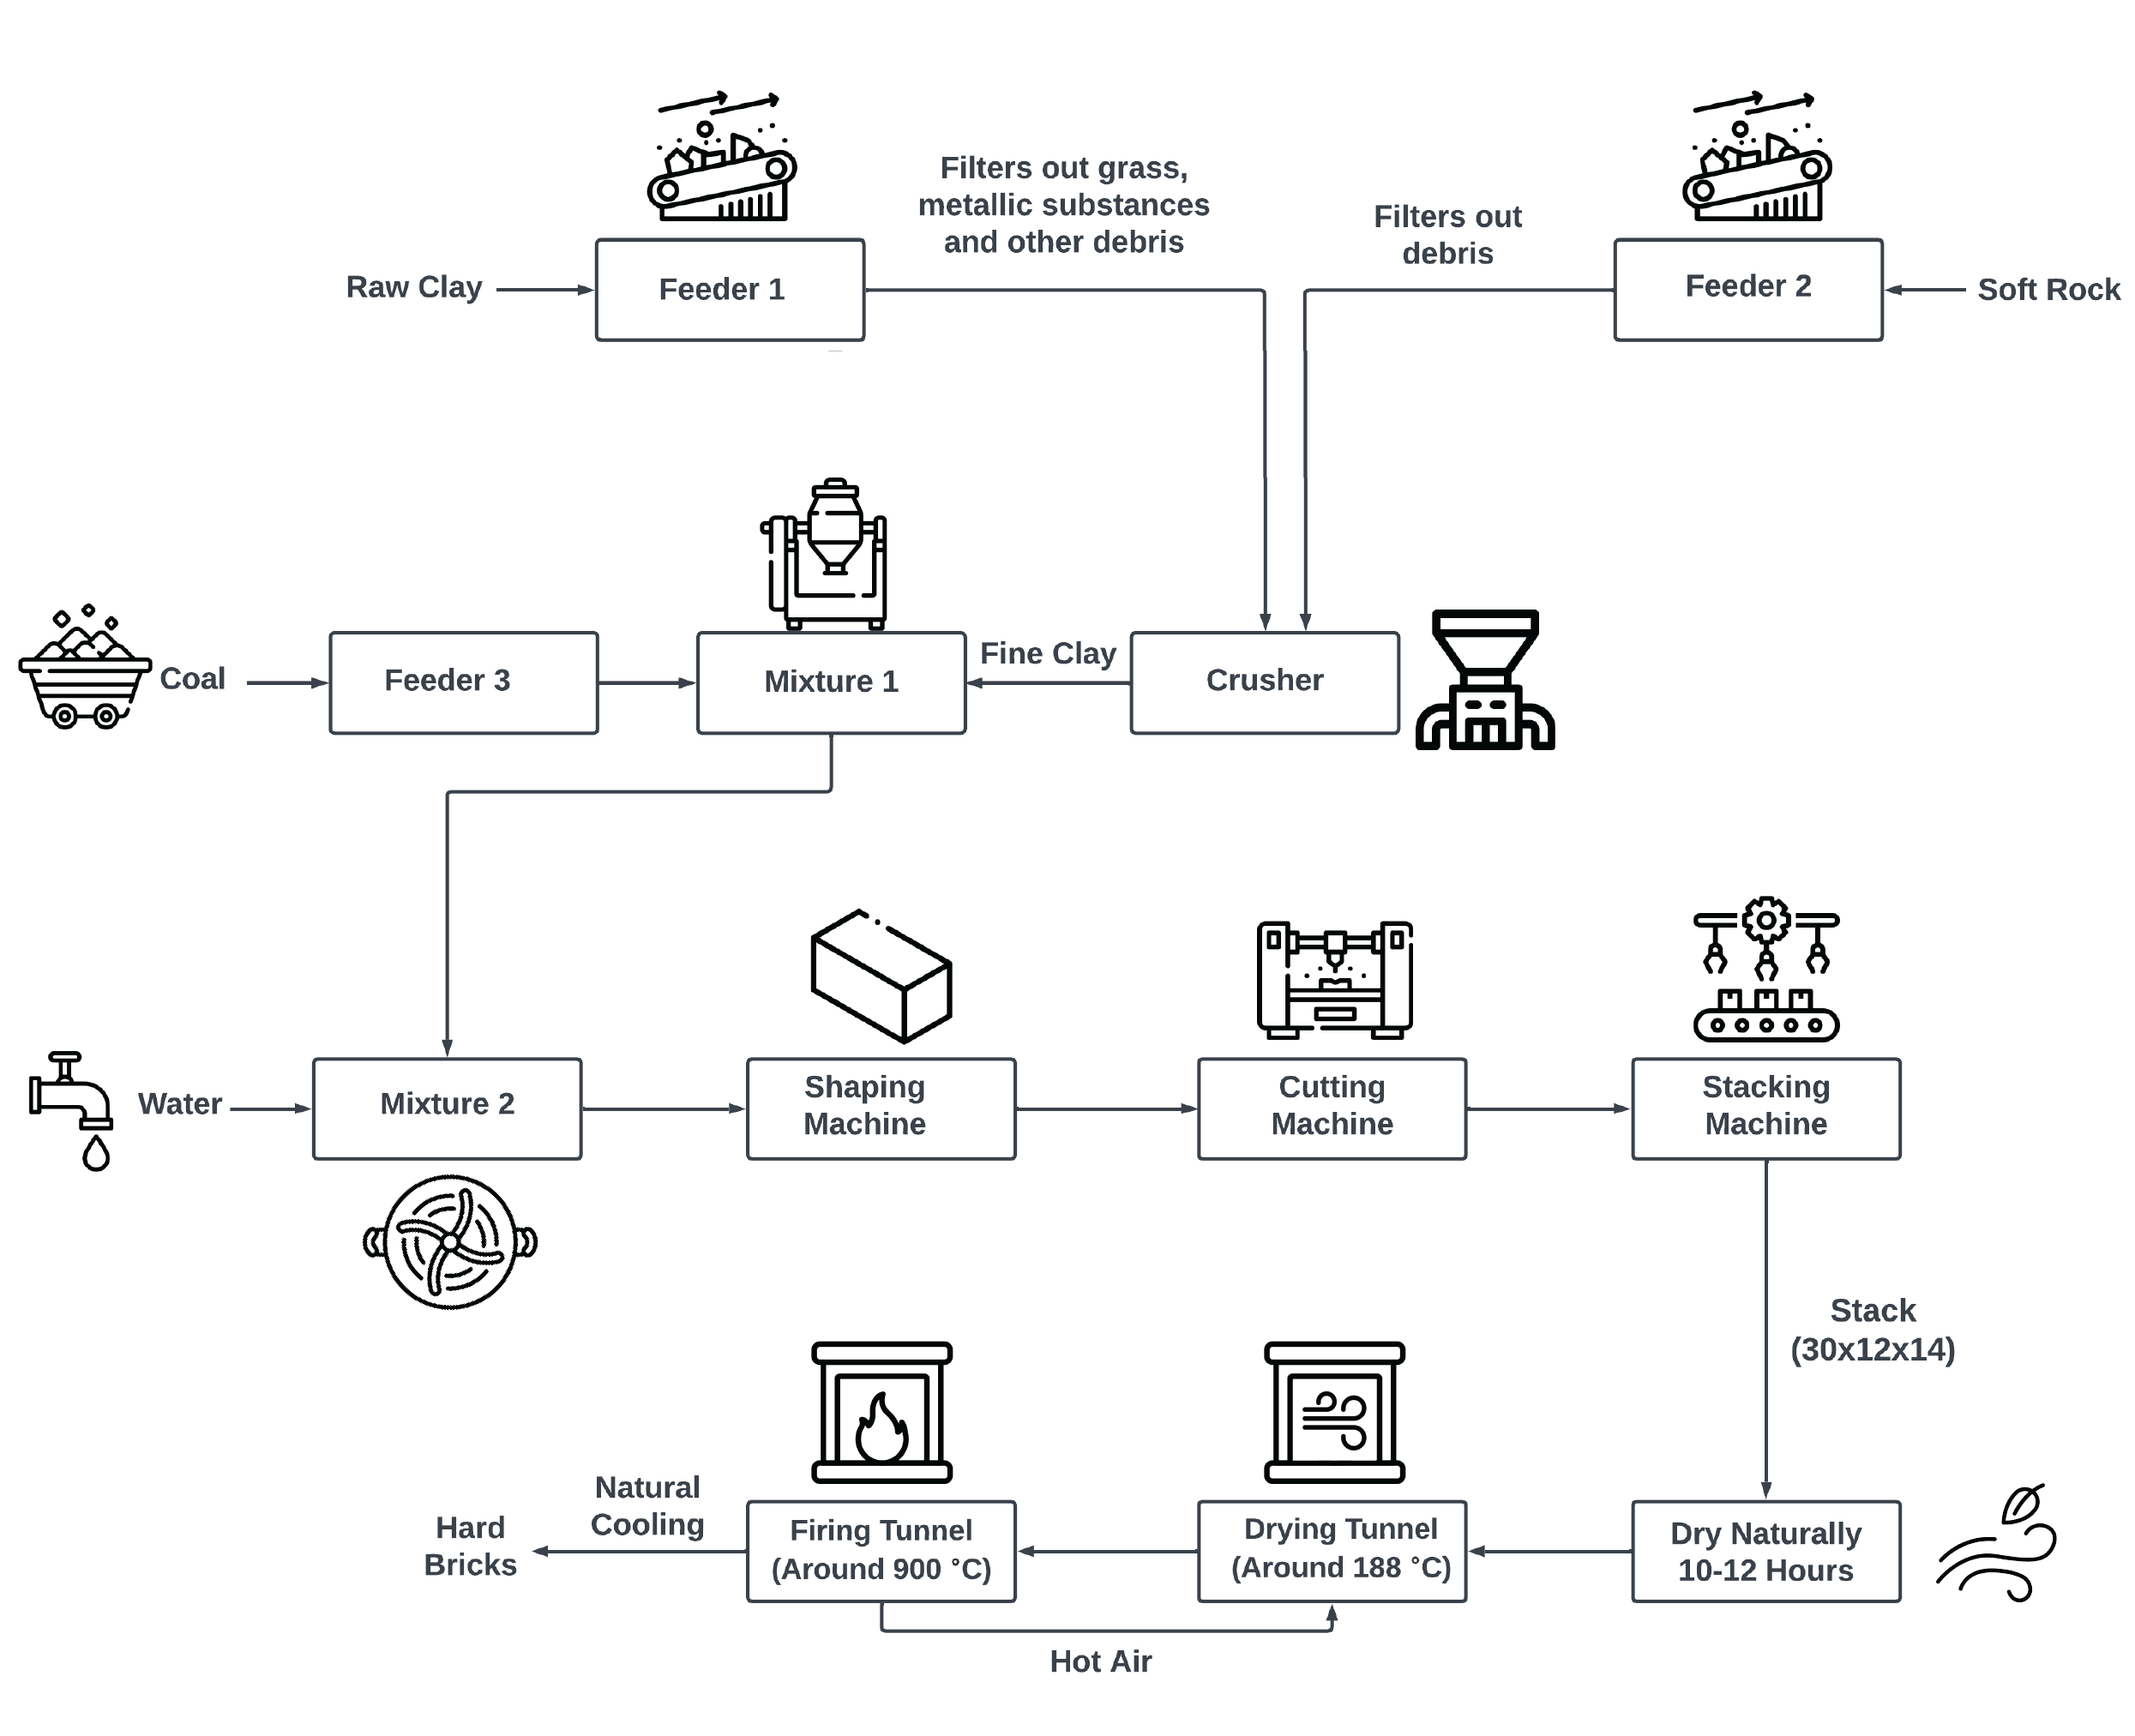
\includegraphics[width=1\textwidth]{img/block diagram.png}
  \caption{Block diagram for brick manufacture process}
\end{figure}

\subsection{Process Flow for Brick Manufacture}
Following are the basic steps of manufacturing bricks:
\begin{enumerate}
\item Clay Preparation
\item Cake Molding
\item Drying
\item Firing 
\item Gradual Cooling
\end{enumerate}

\newpage

\subsubsection{Clay Processing}
First, large chunks of clay are strained using a big strainer. This strainer breaks down the big chunks into smaller pieces. These smaller pieces then pass through a feeder machine. The clay is moved along a rubber conveyor belt to filter out things like grass and unwanted debris. On different parts of the rubber conveyor belt, there are strong magnets placed above to remove any metal from the clay.

Once the clay is roughly filtered, a suitable amount of soft rocks is added to it. The mixture goes through another filtering process. After the filtering is good enough, the mixture is further processed by hammering and thorough mixing to create a finer blend. A small amount of coal is mixed into this fine mixture. This mixture then goes through another feeder, entering mixing machines. Multiple mixing machines ensure proper blending of the clay. Water is also added to the clay in these machines to create a dough-like mixture.

\subsubsection{Cake Molding}
The compact form of clay, molded into brick-like shapes, is known as a "cake." This cake is a vital starting point in the brick-making process. The clay, resembling dough in its texture, is carefully fed through a machine that works to create a consistent and tightly packed structure of clay. This process ensures that the clay is ready for the next steps.

Following this preparation, the clay goes through a precision-cutting phase utilizing a pressure wire cutter. This step results in the clay being divided into smaller lengths, setting the stage for the formation of individual bricks. Each length of clay, once cut by this machine, yields approximately 8 separate bricks.

As these batches of bricks take shape, a specialized mechanism steps in to lift and position them onto a waiting cart. Each cart is made to carry a good number of bricks, fitting in dimensions of about 30 by 12 by 14. The bricks are stacked alternatively to ensure stability. These carts, filled with bricks ready for further processing, are then set into motion by automated machinery.

\subsubsection{Drying}
There are multiple drying steps as explained below:
\subparagraph{Natural Drying}
\begin{adjustwidth}{1.5em}{0em}
\vspace{0.1cm}
  This first stage of natural drying is done right after a cart is fully stacked with bricks. The natural drying process is done for about 12 - 24 hours. This helps to remove moisture from the brick. The natural drying process doesn't completely remove all the moisture.
\end{adjustwidth}



\subparagraph{Preheating}
\begin{adjustwidth}{1.5em}{0em}
In this stage the stacks of brick are preheated to make sure all the moisture are remove from the bricks. It is very crucial to remove moisture from the brick for following reasons:

\vspace{0.1cm}
\textit{Enhanced Strength:}
 Excess moisture weakens the structural integrity of bricks. By \begin{adjustwidth}{1.5em}{0em}removing moisture, the bricks become denser and stronger, making them more resilient and suitable for construction.
 \vspace{0.1cm}
\end{adjustwidth}

\textit{Preventing Cracking:}
 During firing in the kiln, residual moisture can turn into steam, \begin{adjustwidth}{1.5em}{0em}leading to cracks or even explosions in the bricks. Thorough drying prevents such issues by ensuring that moisture is removed before the firing process.
\vspace{0.1cm}
\end{adjustwidth}

\textit{Uniform Firing:}
 Moisture in bricks can cause uneven heating during firing, leading \begin{adjustwidth}{1.5em}{0em}to inconsistencies in color, texture, and strength. Properly dried bricks ensure a more uniform and desirable end product.
 \vspace{0.1cm}
\end{adjustwidth}

\textit{Reduced Shrinkage:}
 Moisture causes bricks to shrink during the firing process, which \begin{adjustwidth}{1.5em}{0em}can result in variations in size and shape. Drying minimizes shrinkage, leading to more standardized and consistent bricks.
\vspace{0.1cm}
\end{adjustwidth}

\textit{Efficient Firing:} Drier bricks require less energy to heat during firing, making the \begin{adjustwidth}{1.5em}{0em}process more energy-efficient and cost-effective.
\vspace{0.1cm}
\end{adjustwidth}
\end{adjustwidth}
\vspace{0.1cm}

\subsubsection{Firing}
Following the completion of the preheating stage, the stack of bricks is introduced into the firing tunnel. Here, the bricks are subjected to firing at temperatures of approximately 900°C. The temperature range within the tunnel can fluctuate between 900°C and 950°C, influenced by the surrounding environmental conditions. The firing process persists for roughly an hour per stack of bricks. Throughout this duration, the coal contained within the bricks undergoes combustion, leading to chemical changes. Notably, the iron content in the bricks transforms into iron oxide, imparting orange hue to the bricks.

\vspace{0.1cm}
The temperature within the tunnel is monitored from a designated room. A monitoring system displays the temperature readings from various segments of the Drying and Firing Tunnel. For temperature measurement, Type K thermocouple sensors are positioned above the tunnel, capable of gauging a range up to 0-1200\degree C. Additionally, each tunnel features approximately 9 small openings for direct monitoring. Within the tunnel, two fans play essential roles—one functions as an exhaust fan, while the other facilitates the circulation of air into the drying tunnel. The heat generated in the firing tunnel is channeled into the drying tunnel to preheat the bricks. The velocity of the fan is regulated using a VFD (Variable Frequency Drive), a motor controller capable of altering motor speed and consequently adjusting fan speed.

\subsubsection{Gradual Cooling and Loading}
After the bricks undergo the heating process, they need to cool down gradually. This cooling phase takes place by letting the bricks interact with the air around them. This natural cooling is crucial to prevent the bricks from becoming too brittle or prone to cracking. It allows the bricks to adjust to the surrounding temperature and conditions in a balanced way.

Once the cooling process is complete and the bricks have reached a stable state, they are prepared for transportation. Loading the cooled bricks onto transportation vehicles requires careful handling to avoid any damage that could weaken the bricks. This loading process ensures that the bricks maintain their strength and structural integrity during transit.